\subsection{Buildings on the ground}
\paragraph{}
In this example, a few buildings on different layers under gravity of soils are considered.
Fig.~\ref{qdt_fig:ex_building_geo} illustrates the geometry and boundary condition of the problem and Fig.~\ref{qdt_fig:ex_building_mat} shows the material property of the problem.
Fig.~\ref{qdt_fig:ex_building_CAD} represents the design file in AutoCAD.
Fig.~\ref{qdt_fig:ex_building_mesh} and Fig.~\ref{qdt_fig:ex_building_stress} plot the mesh and the von-mises stress correspondingly.
\begin{figure}
    \centering
    \scalebox{0.4}{
        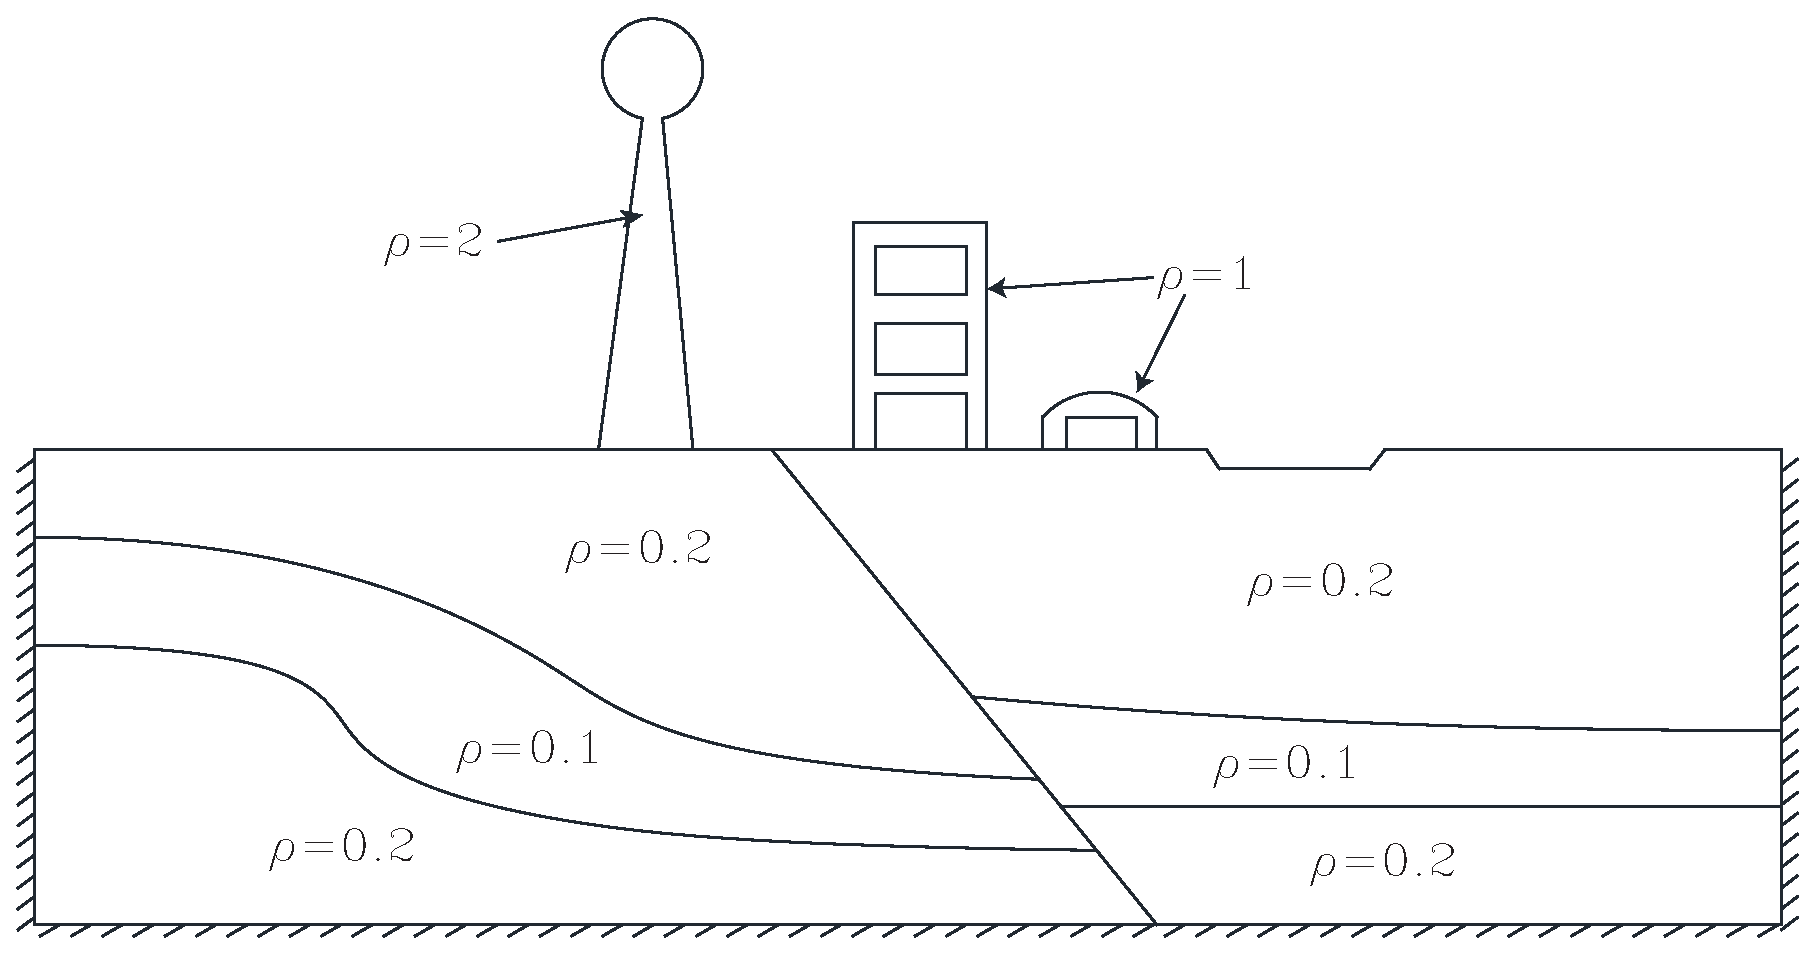
\includegraphics{quadtree/ex_images/ex_building_geo.eps}
    }
    \caption{Geometry and boundary condition of the problem}
    \label{qdt_fig:ex_building_geo}
\end{figure}

\begin{figure}
    \centering
    \scalebox{0.4}{
        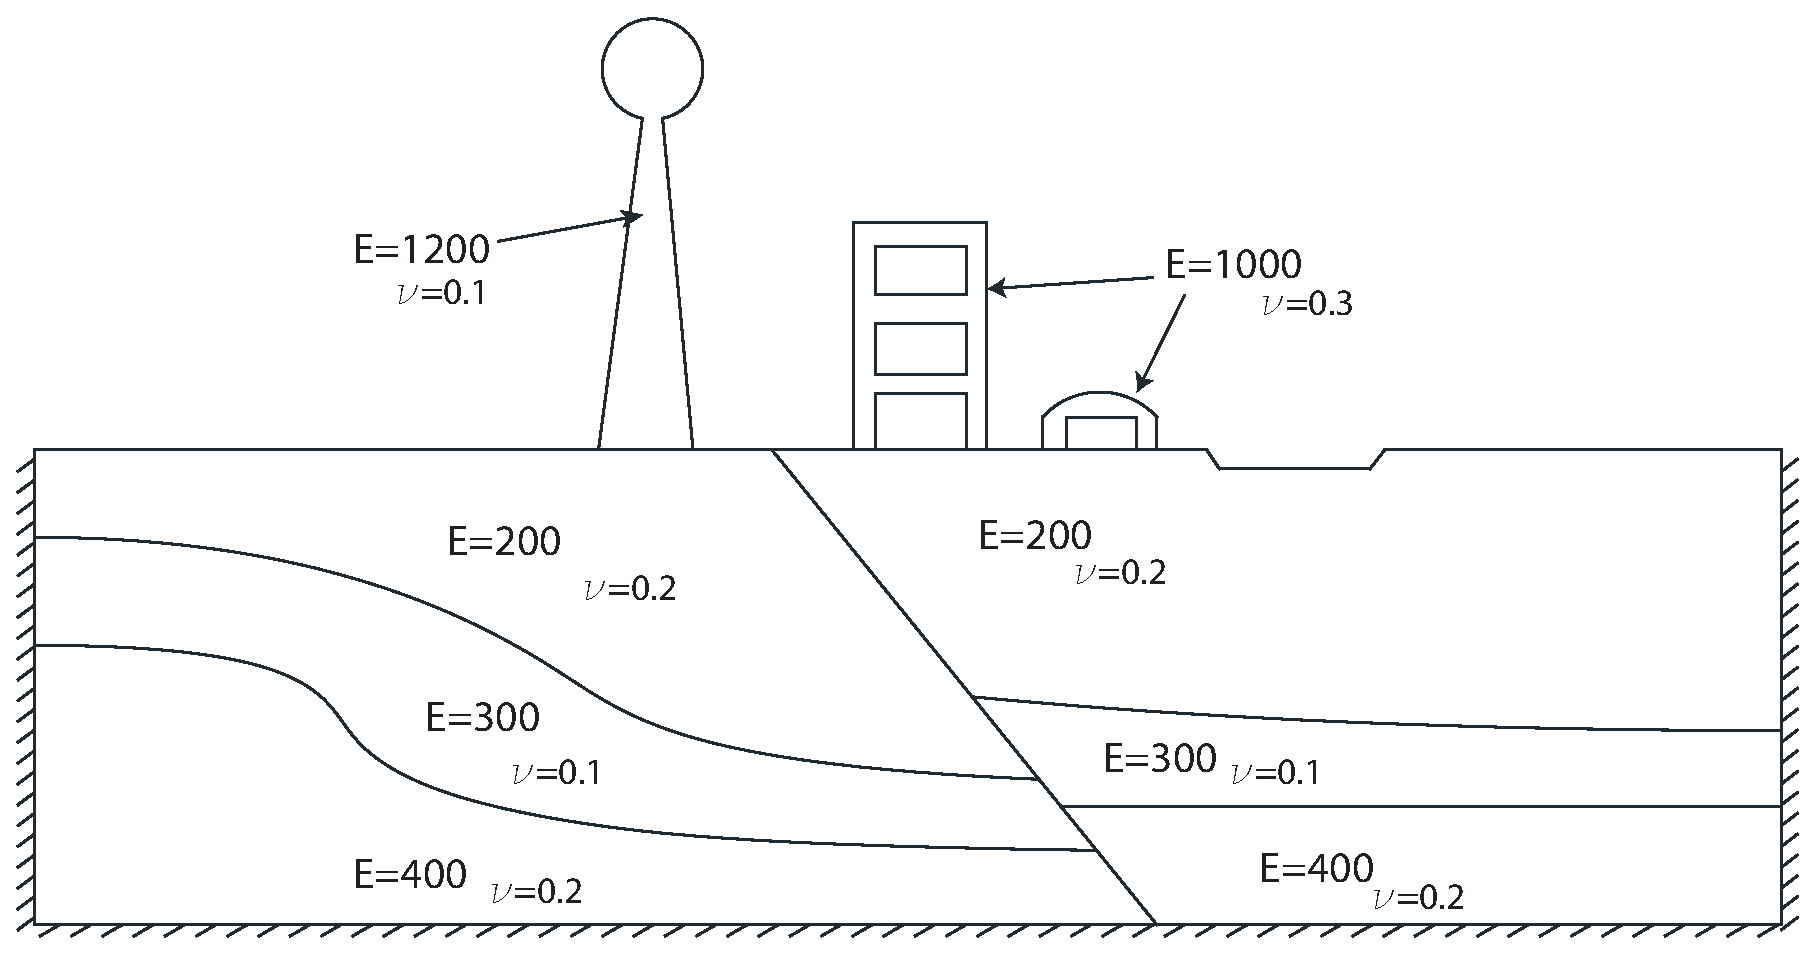
\includegraphics{quadtree/ex_images/ex_building_material.eps}
    }
    \caption{Geometry and boundary condition of the problem}
    \label{qdt_fig:ex_building_mat}
\end{figure}

\begin{figure}
    \centering
    \scalebox{0.3}{
        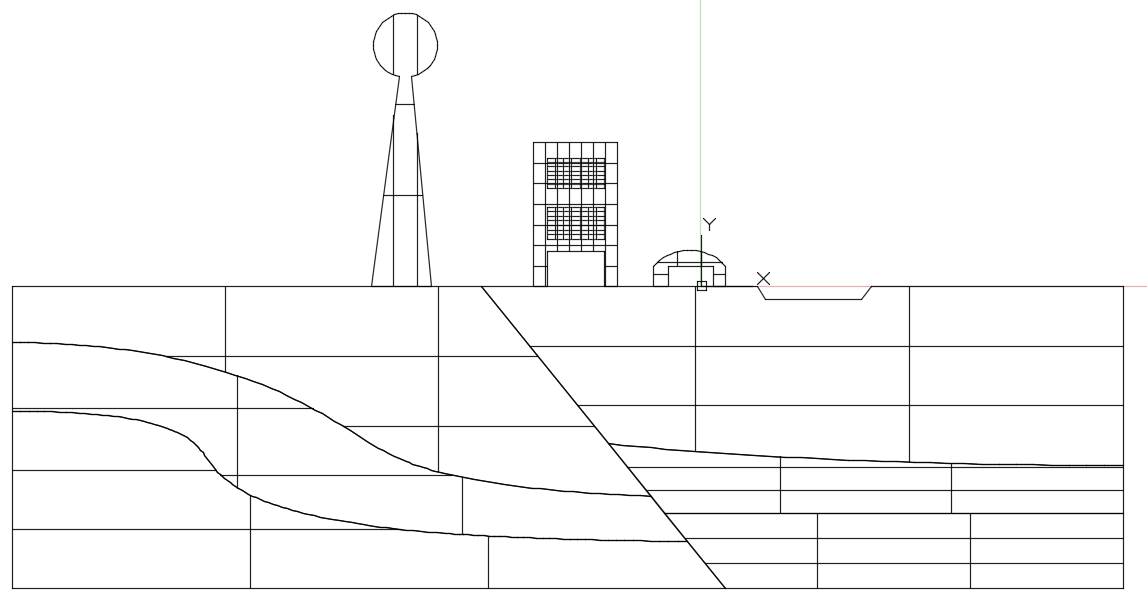
\includegraphics{quadtree/ex_images/ex_building_autocad.png}
    }
    \caption{Design in AutoCAD}
    \label{qdt_fig:ex_building_CAD}
\end{figure}

\begin{figure}
    \begin{subfigure}[b]{1\linewidth}
        \centering
        \scalebox{0.4}{
            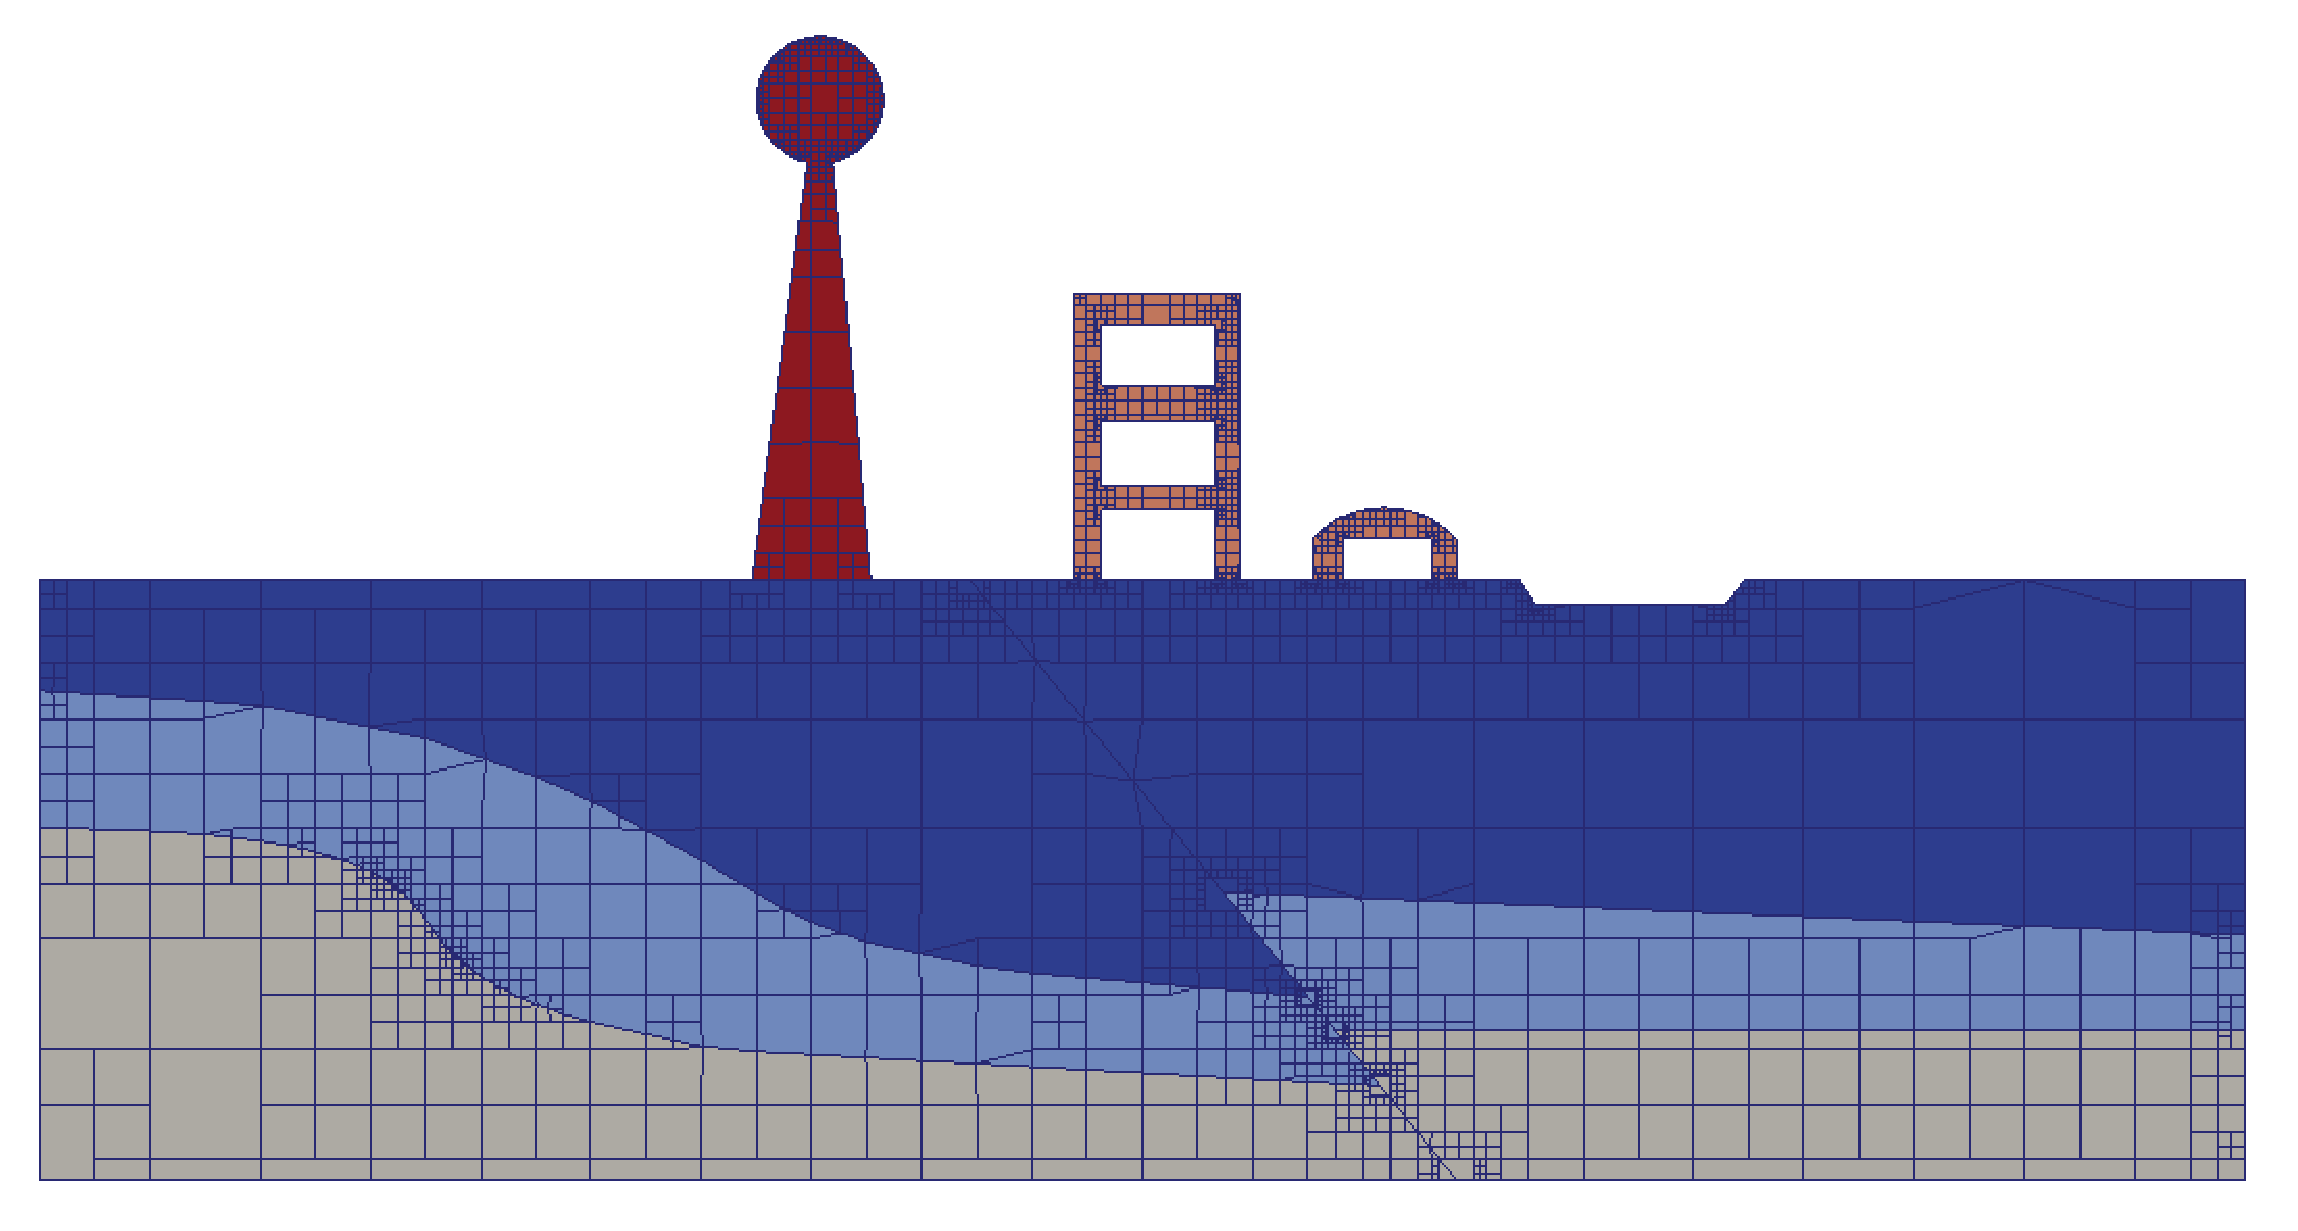
\includegraphics{quadtree/ex_images/ex_building_mesh.eps}
        }
        \caption{Mesh}
    \end{subfigure}\\
    \begin{subfigure}[b]{1\linewidth}
        \centering
        \scalebox{0.4}{
            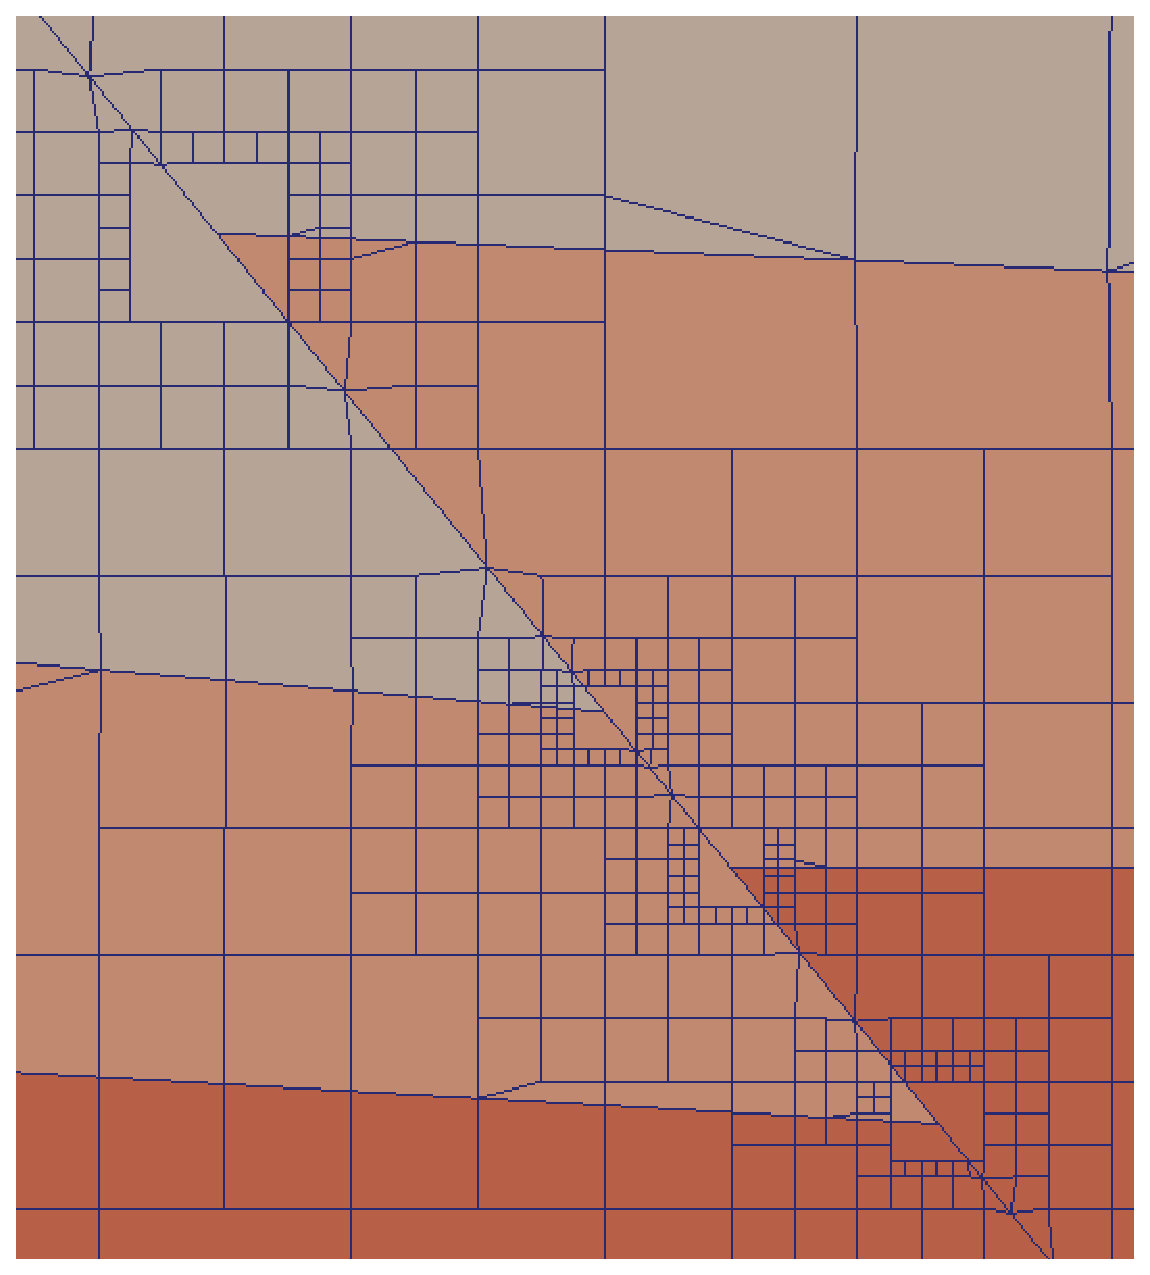
\includegraphics{quadtree/ex_images/ex_building_mesh_enlarge.eps}
        }
        \caption{Mesh at the sharp corner}
    \end{subfigure}
    \caption{Meshing of the buildings}
    \label{qdt_fig:ex_building_mesh}
\end{figure}

\begin{figure}
    \centering
    \scalebox{0.4}{
        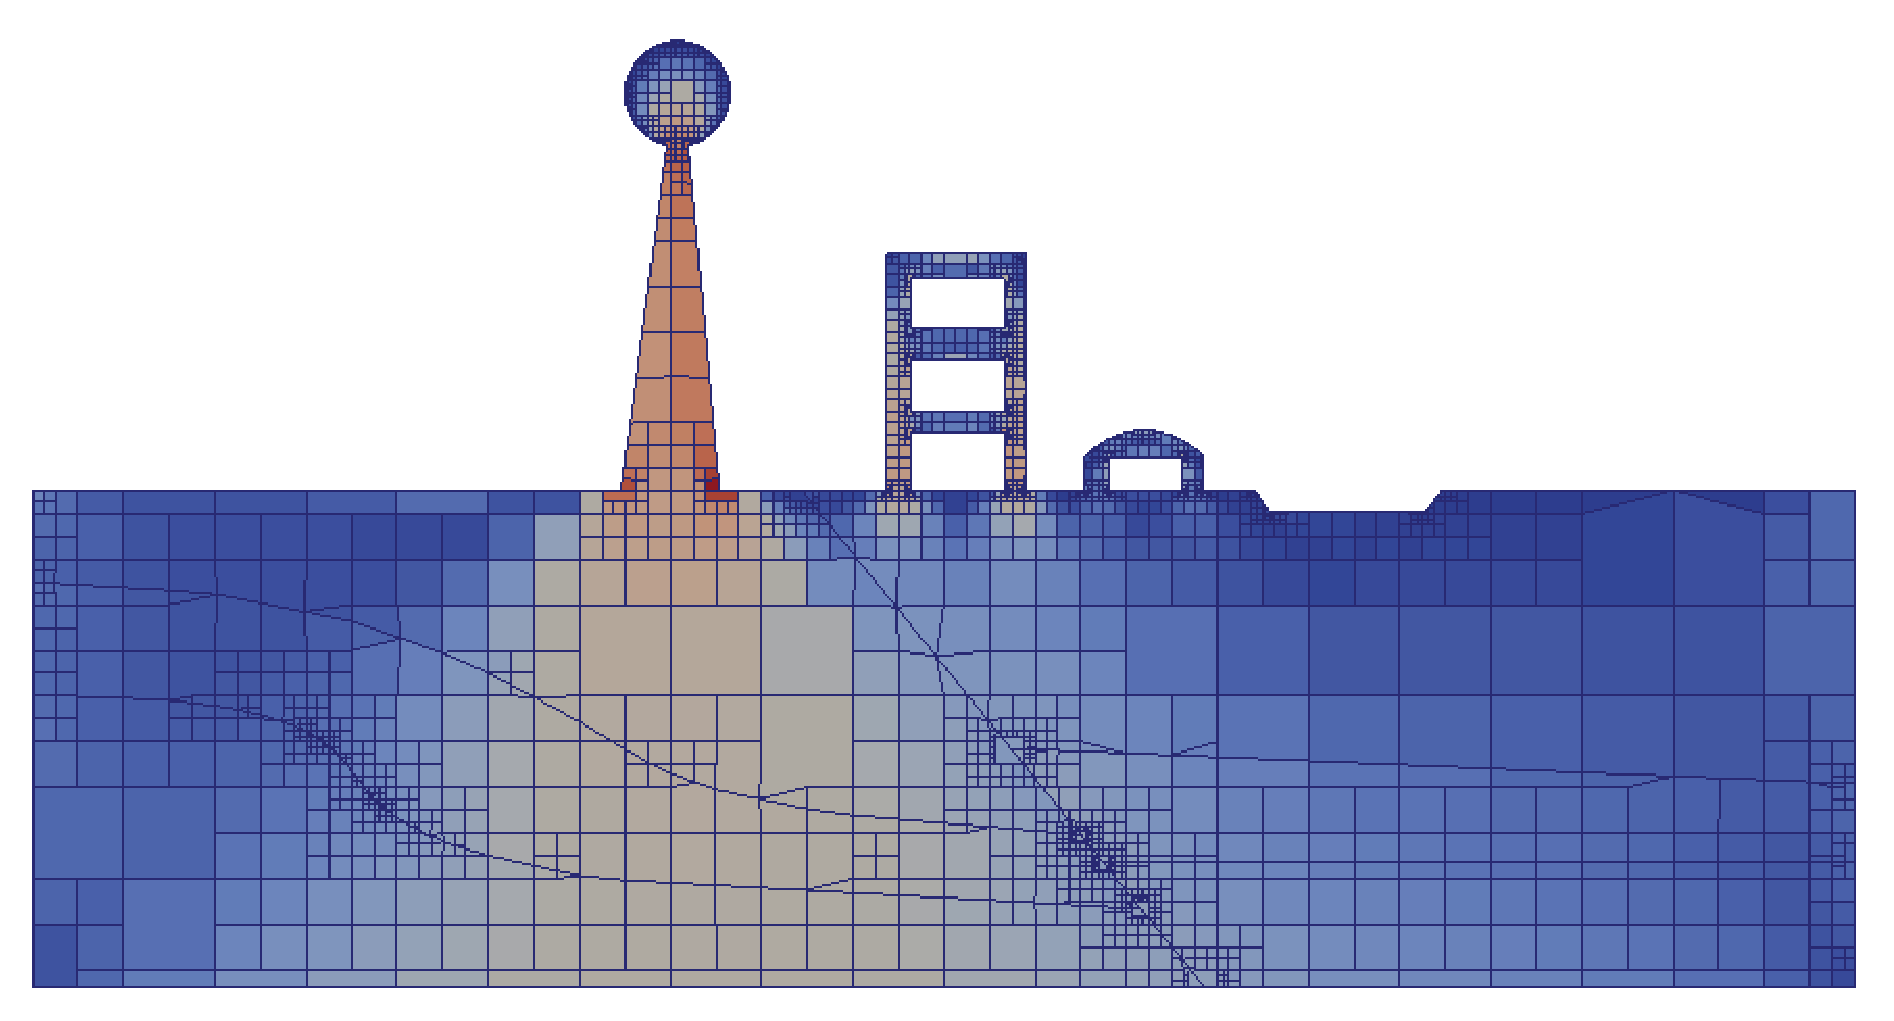
\includegraphics{quadtree/ex_images/ex_building_stress.eps}
    }
    \caption{Von-mises stress contour for the buidlings on the ground}
    \label{qdt_fig:ex_building_stress}
\end{figure}
